\chapter{Experiments}
\section{Environments}

First environment used for evaluation is the \emph{Slimevolley} environment. The Slimevolley environment \cite{slimevolleygym} is based on a game called "Slime Volleyball" created by an unknown author. The agent's task in this environment is to get the ball to hit ground on the opponent's side to make the oponent lose a life. The opponent is controlled by a small, 120-parameter, pre-trained neural network. \cite{ha2015slimevolley}

Each agent has 5 lives in the beginning and the episode ends after 3000 steps or when either agent loses or their lives, whichever comes first. The agent receives a reward of $+1$ point when the opponent loses a life and $-1$ if it loses the life. In addition to this, for each survived timestep, the agent receives $+0.01$  reward. State is represented as a vector with 12 entries, $x$ and $y$ positions and respective velocities of the agent, opponent and the ball. Actions are represented as a vector with 3 entries, one for each action that the agent can do, jump, go forward or go backward. The agent will perform an action when the appropriate value is higher than 0.

\begin{figure}[h]
    \caption{Screenshot of Slimevolley environment}
    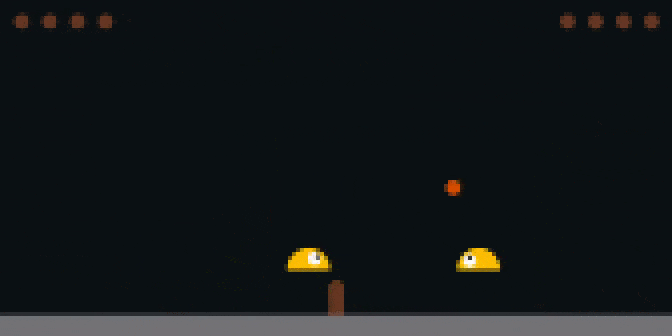
\includegraphics[width=0.8\textwidth]{img/slimevolley.png}
\end{figure}

Second environment is a \emph{Cartpole-swingup} environment. It is inspired by classic reinforcement learning benchmark task, pole-balancing. In this task one end of a pole is attached to a card which moves left and right and the goal is to keep the pole upright. In the original the episode ends when the pole is tilted too much off its neutral position. However in this version the pole is able to rotate $360^\circ$ and the episode ends only if the cart goes out of bounds or 1000 timesteps goes past.

The physics of the pole is controlled by equations specified for "Pendullum Swing-up" in PILCO software package \cite{pilco2013}. Reward is given based on how far is the cart from centre (closer is better) and what is the angle of the pole (more upright is better). State is represented with a 4-entry vector containing the position of the cart, its velocity, sine and cosine of the pole's angle and its angular velocity while action is a number from -1 to 1 which represents force which is applied, in either direction, to the cart.

\begin{figure}[h]
    \caption{Screenshot of Cartpole-swingup environment}
    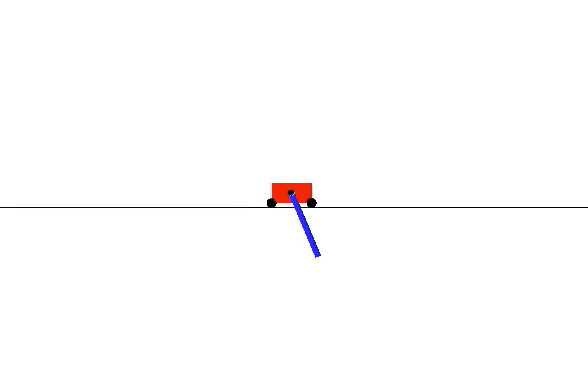
\includegraphics[width=0.8\textwidth]{img/cartpole.png}
\end{figure}
% 
The behavioural characteristics is calculated similarly in both environments, inspired by approach used in \cite{Inden2013} for classic Cartpole problem. For Slimevolley the $x$-coordinate of the controlled agent at timesteps 10, 30, 100, 300, 1000 and 3000 is taken and in Cartpole environment the $x$-coordinate of the cart at timesteps 5, 10, 50, 100, 500 and 100 is taken. If the environment doesn't reach that state a 0 is filled in. This slightly differs from the implementation outlined in \cite{Inden2013}. Then simple Euclidean norm is used to calculcate distance between two such characteristics.

Controlled agents's policies are represented with small feed-forward neural networks, for Cartpole 1-layer neural network with 5 inputs, 10 neurons in middle layer and one output neuron and $\tanh$ activation function applied to output of all neurons. Slimevolley has a bigger network, 12 input neurons, two layers with 20 neurons and 3 output neurons with $\tanh$ activation function. 

\section{Experiments}

There were several experiments run in each environment. All experiments were run 10 times with different starting seeds for 1000 or 900 (in case of novelty based algorithms due to memory contraint on system where experiments were run) generations with population of 90 and 3 episodes per evaluation. The 6 six methods that were tried are:
\begin{itemize}
    \item CMA-ES, 
    \item PEGP,
    \item OpenAI ES,
    \item NS-ES, 
    \item NSR-ES and
    \item NSRA-ES.
\end{itemize}

For CMA-ES, the only parameter was $\sigma_{init}$ which controls the initial standard deviation and it was set to 0.1. PGPE had $\sigma_{init}$ 0.1 and other parameters controlling the standard deviation set to 0.2, 0.999, 0.01 and 0.2 for learning rate, rate of decay, limit and maximal change. OpenAI-ES started with $\sigma$ 0.1, rate of decay 0.999 and limit 0.01. Novelty search based algorithm had fixed $\sigma$ (because it doesn't make sense to change it since there are more individuals) of 0.1 and used 5 as $k$ in k-nearest neighbours and metapopulation with size 5. In addition to that NSRA-ES waited 10 steps before increasing the ratio of novelty in the gradient by 0.05. All algorithms, except for CMA-ES, used the Adam \cite{kingma2017adam} optimiser, with learning rate 0.1. In all presented graphs a median is shown along with the first and third quartile.

\subsection{Slimevolley}

The experiments have shown that this environment is quite challenging to solve. Only CMA-ES has managed to get good results in the 10 runs included in the experiment. Since the reward received by CMA-ES caps at 30 it would suggest that the agent didn't learn to beat the opponent but only to defend well enough. However during development OpenAI-ES has managed to get some good results as well but it was strongly sensitive to seed, equalling the performance of CMA-ES in some runs while not improving at all in others. Novelty search-based methods did fail as well on this problem while intuitively they should have a higher chance of producing good results as they are able to explore in multiple directions at once thus have higher probability of going in the right direction. Bad performance by NS-ES was expected and in accordance with \cite{conti2018}. However both NSR-ES and NSRA-ES did not perform well either which points to either badly designed novelty or suboptimal hyperparameter setting. 

\begin{figure}[H]
    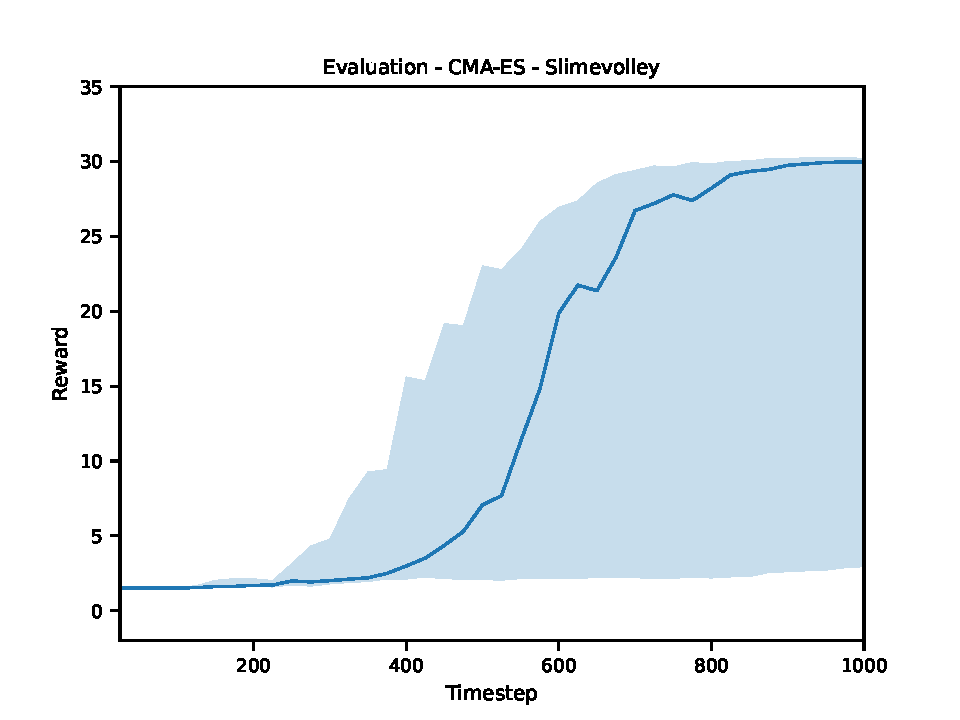
\includegraphics[width=0.9\textwidth]{img/eval-slime-cmaes.pdf}
\end{figure}
\begin{figure}[H]
    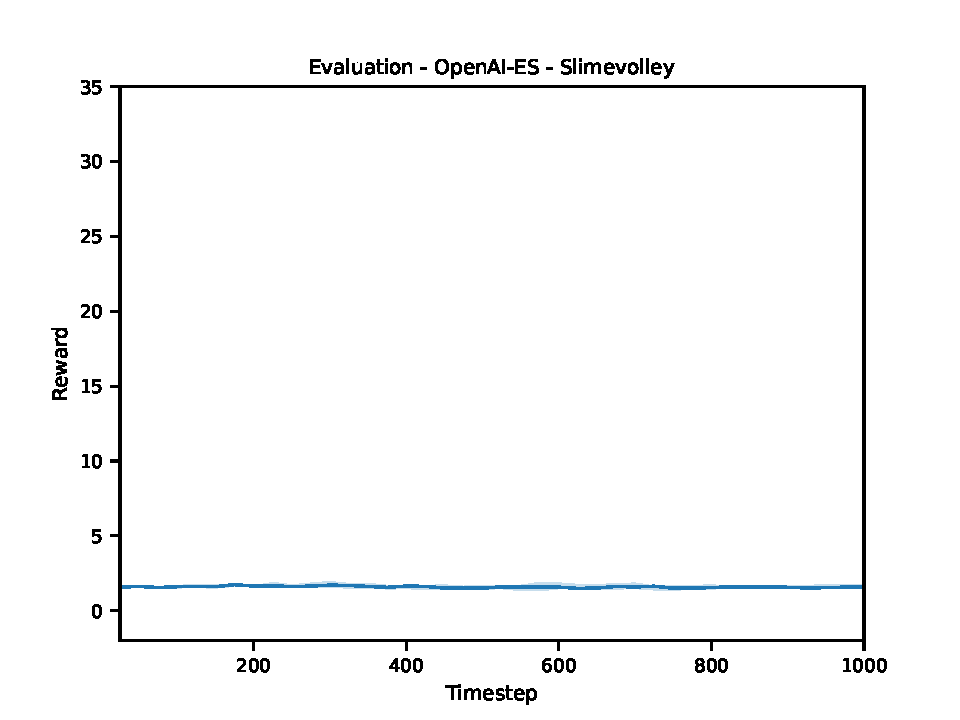
\includegraphics[width=0.9\textwidth]{img/eval-slime-open.pdf}
\end{figure}
\begin{figure}[H]
    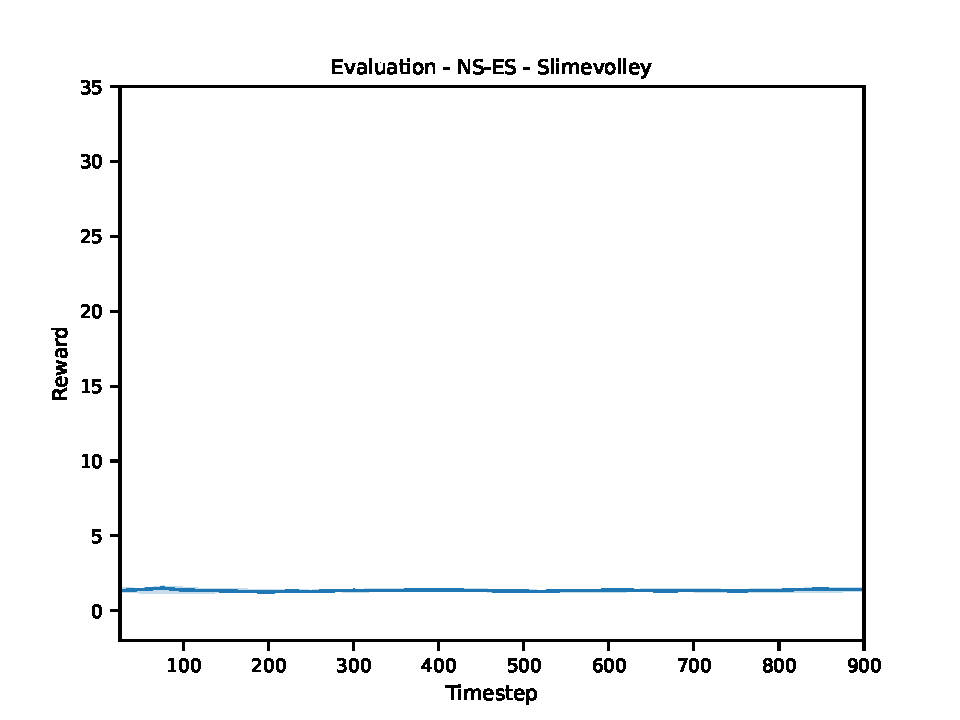
\includegraphics[width=0.9\textwidth]{img/eval-slime-nses.pdf}
\end{figure}
\begin{figure}[H]
    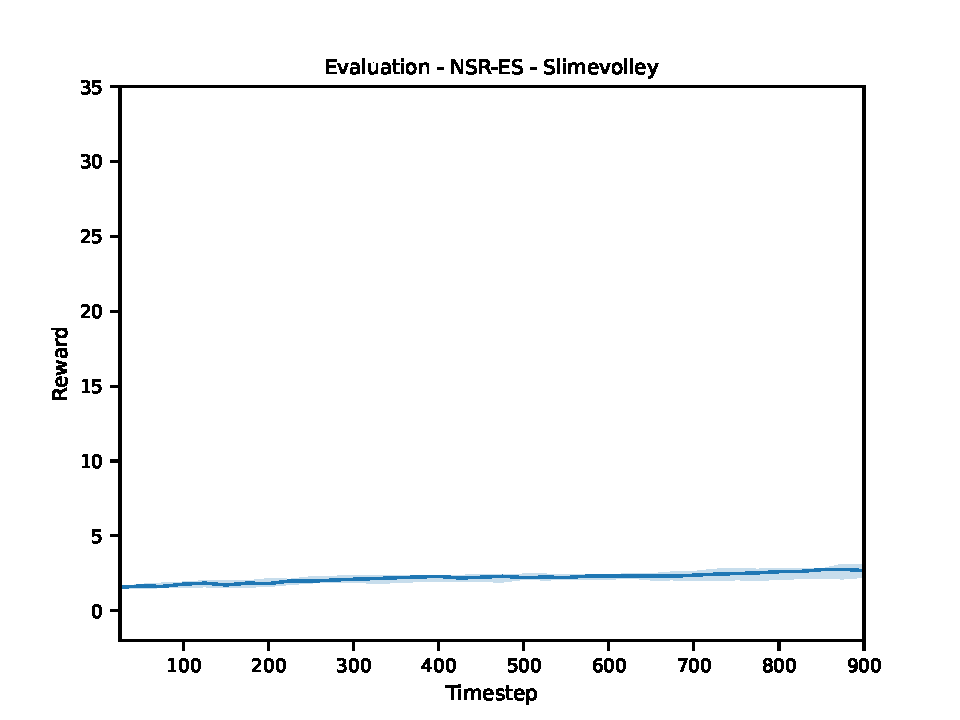
\includegraphics[width=0.9\textwidth]{img/eval-slime-nsres.pdf}
\end{figure}
\begin{figure}[H]
    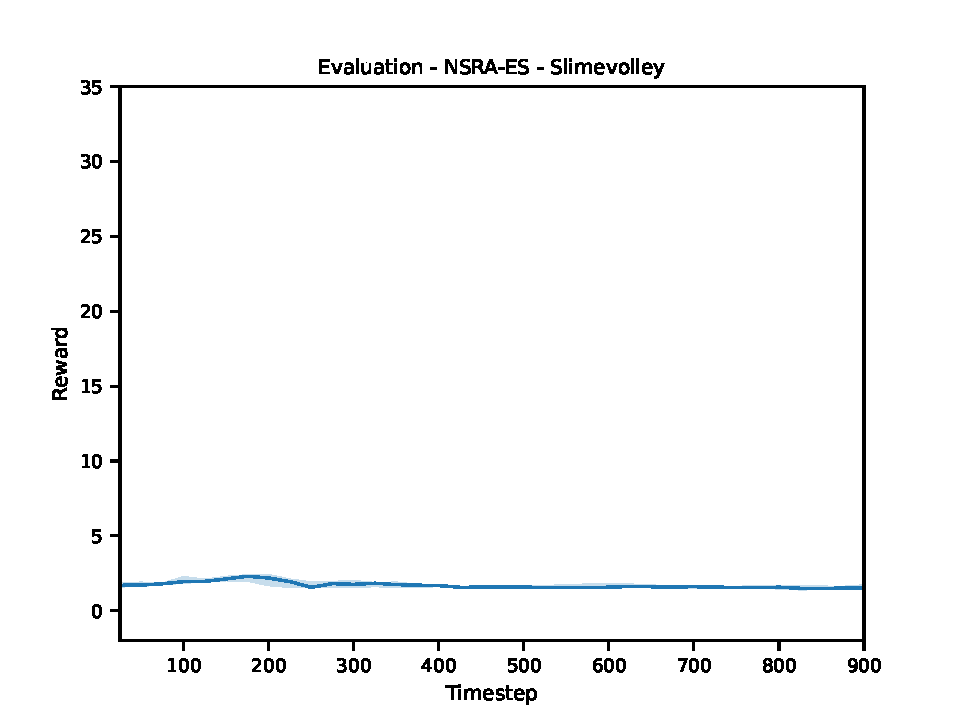
\includegraphics[width=0.9\textwidth]{img/eval-slime-nsraes.pdf}
\end{figure}
\begin{figure}[H]
    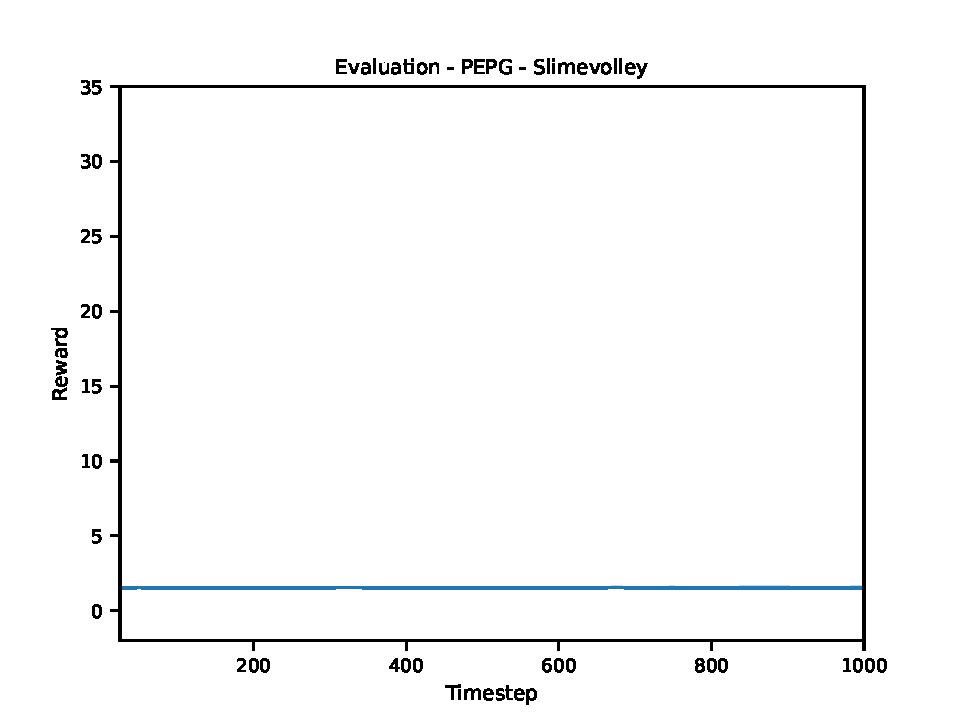
\includegraphics[width=0.9\textwidth]{img/eval-slime-pepg.pdf}
\end{figure}
\newpage

\subsection{Cartpole-swingup}

This environment has proven to be significantly less challenging than Slimovolley. Both OpenAI-ES and CMA-ES have managed to solve it but CMA-ES seems to have a significant performance dropoff in later generations. Closer inspection of data from traning has shown that in some cases the trainig gets stuck at values around 925 with parameters slowly growing in magnitude before completely exploding and performance dropping off. Bad performance from NS-ES was expected as it has no incetive to pursue better performance. NSR-ES slowly and steadily improves and the trajectory suggests that it would improve further given more time. This is most likely thanks to having 1:1 ratio of fitness and novelty therefore the the search for novelty slows down the search for improvement. In case of NSRA-ES a fast improvement can be seen in the beginning however as the weight of novelty slowly increases the algorithm starts to perform similarly to NS-ES. This behaviour can be probably avoided with either better hyperparameter tuning or better novelty calculation.


\begin{figure}[H]
    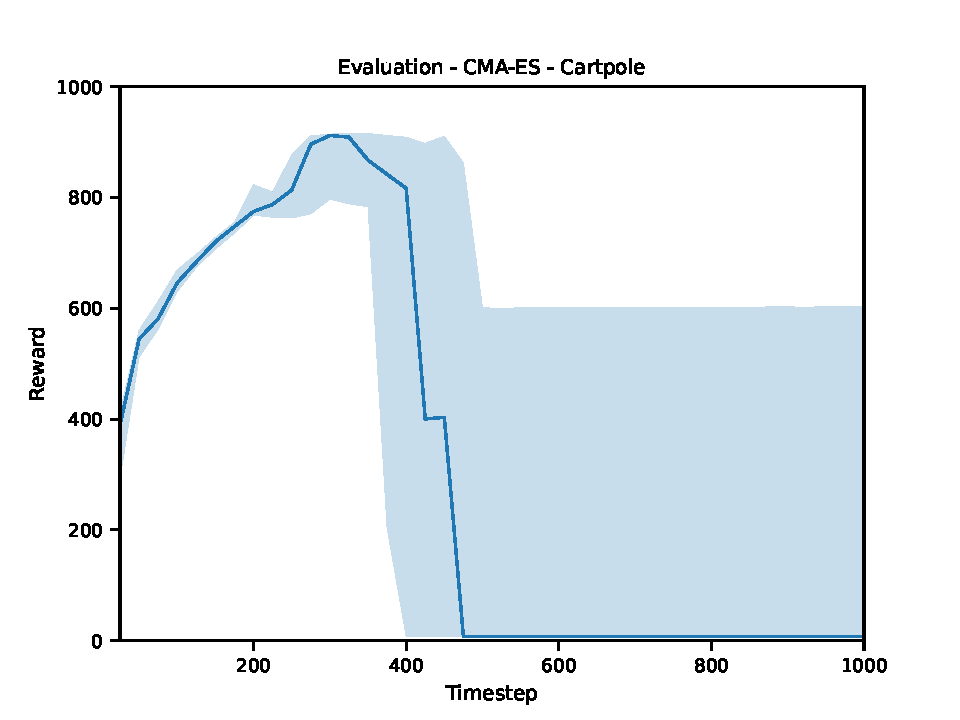
\includegraphics[width=0.9\textwidth]{img/eval-cart-cmaes.pdf}
\end{figure}
\begin{figure}[H]
    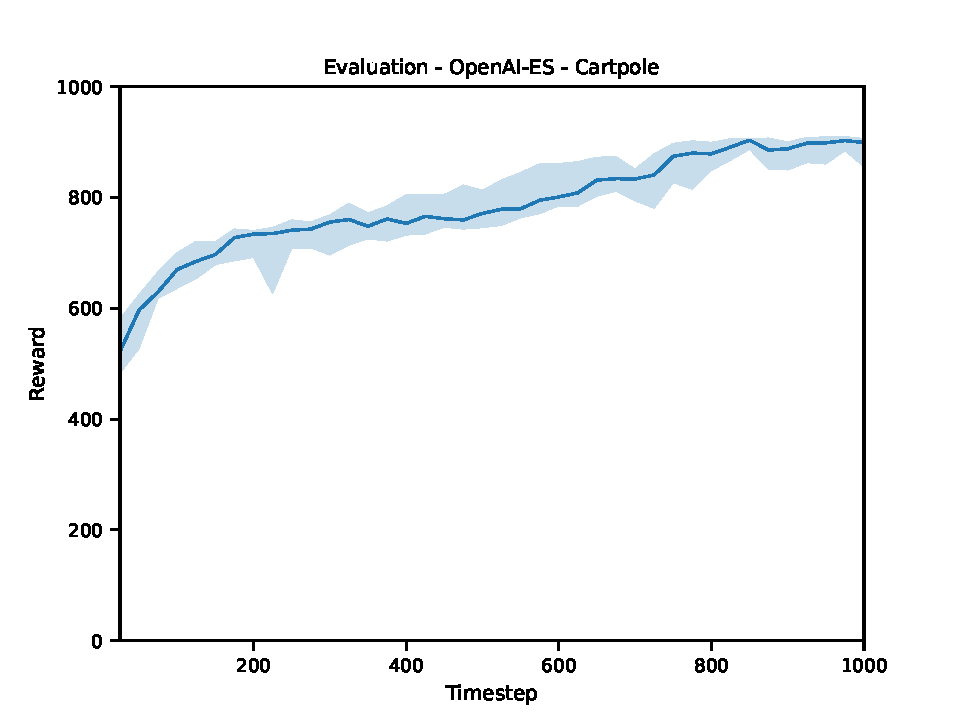
\includegraphics[width=0.9\textwidth]{img/eval-cart-open.pdf}
\end{figure}
\begin{figure}[H]
    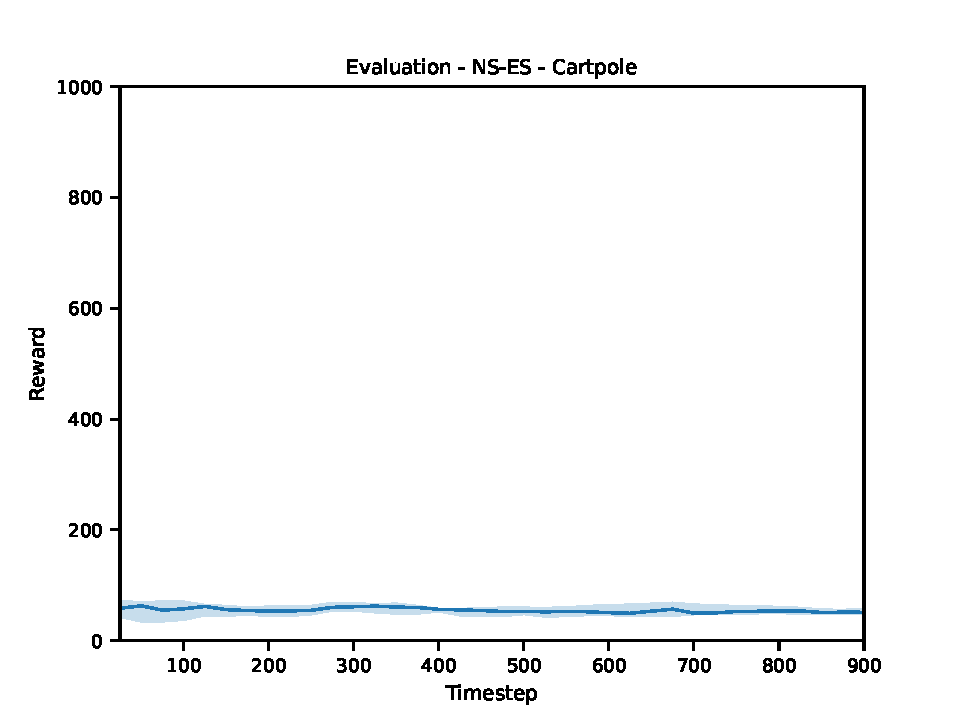
\includegraphics[width=0.9\textwidth]{img/eval-cart-nses.pdf}
\end{figure}
\begin{figure}[H]
    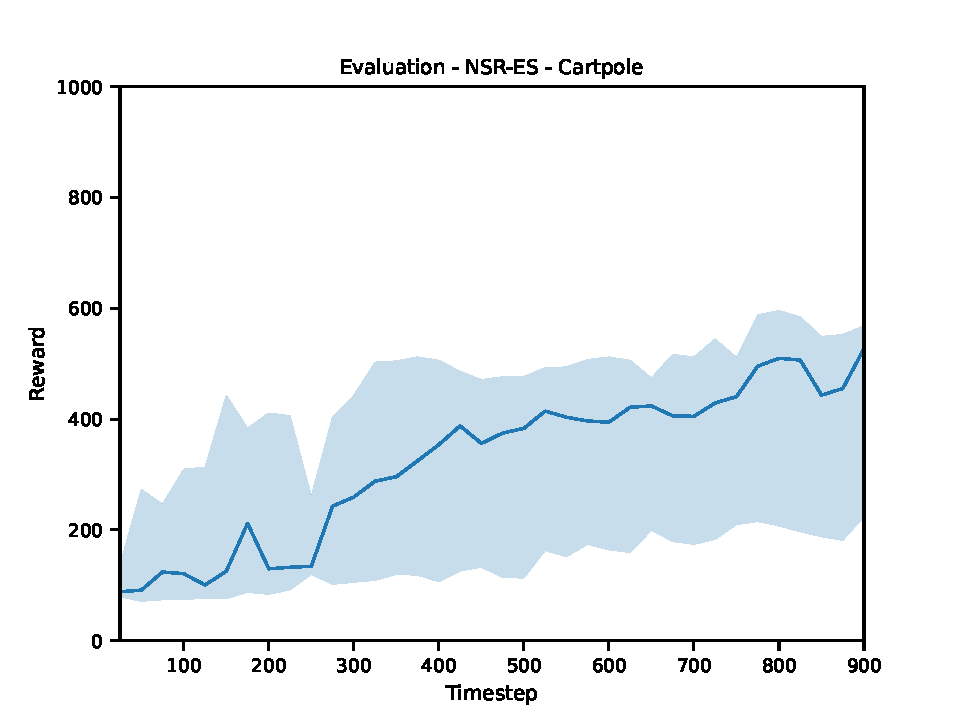
\includegraphics[width=0.9\textwidth]{img/eval-cart-nsres.pdf}
\end{figure}
\begin{figure}[H]
    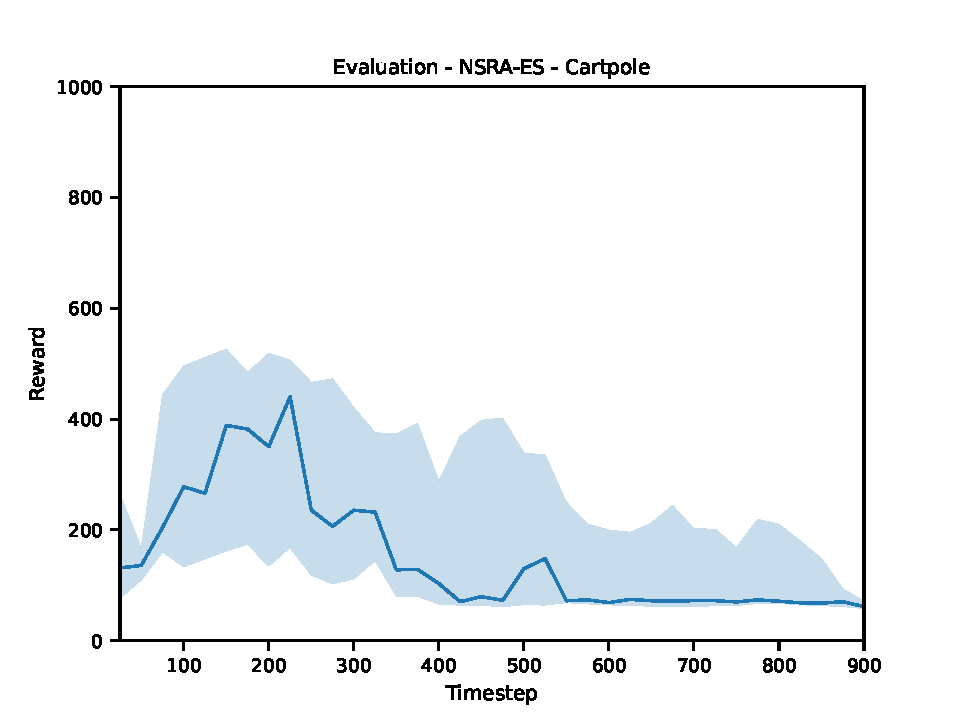
\includegraphics[width=0.9\textwidth]{img/eval-cart-nsraes.pdf}
\end{figure}
\begin{figure}[H]
    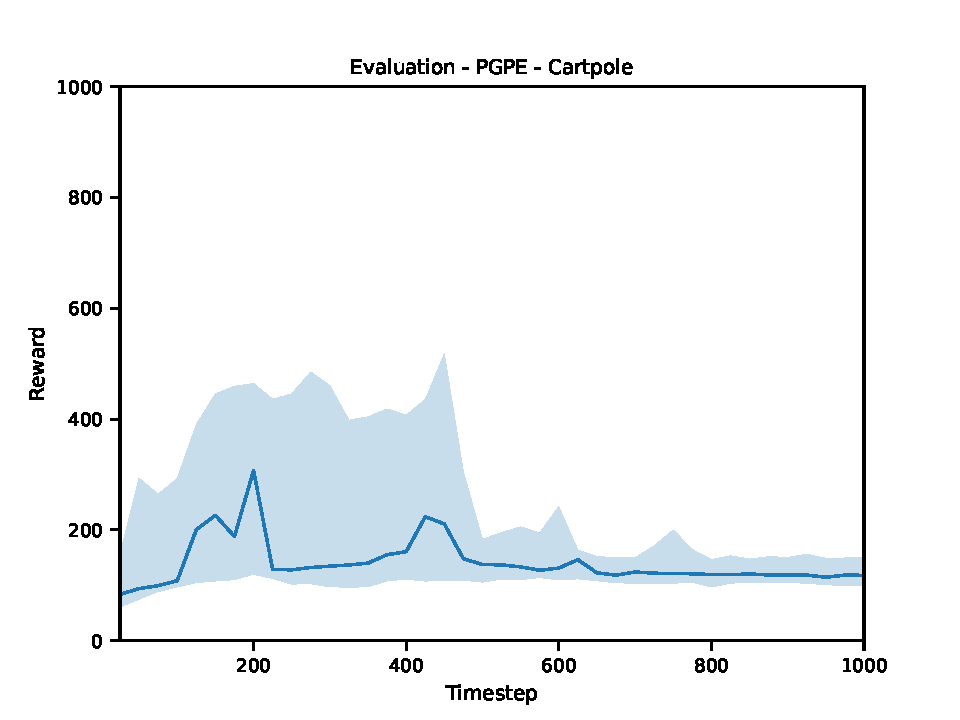
\includegraphics[width=0.9\textwidth]{img/eval-cart-pepg.pdf}
\end{figure}
